\documentclass[a4paper,times,12pt]{article}
%\usepackage{indentfirst}
\usepackage{amsmath}
\usepackage{graphicx}
\usepackage{float}
\usepackage{setspace}
%\usepackage{svg}
\usepackage{subcaption}
%\usepackage{minted}
\onehalfspacing
\usepackage[top=2.5 cm, bottom=2.5 cm, left=4 cm, right=2.5 cm]{geometry}
%\usepackage{hyperref}
\usepackage{algorithm}
\usepackage[noend]{algpseudocode}

\makeatletter
\def\BState{\State\hskip-\ALG@thistlm}
\makeatother

\newcommand\tab[1][0.5cm]{\hspace*{#1}}

\setlength\parindent{0pt}

\begin{document}

\begin{titlepage}
\begin{center}
\vspace*{1cm}
\underline{\textbf{\Large ISTANBUL TECHNICAL UNIVERSITY}} \\[10 pt]

\underline{\textbf{\large FACULTY OF SCIENCE AND LETTERS}} \\[15 pt]

\textbf{\large Graduation Project} \\
\vspace{1.8 cm}

\includegraphics[scale=1.2]{itu_logo.pdf} \\
\vspace{1.8 cm}
%\textbf{\large Machine Learning and Nonlinear Schr{\"o}dinger Equation} \\[5 pt]
\textbf{\large Machine Learning and Non-linear Schr{\"o}dinger Equation} \\[5 pt]
\textbf{H{\"u}seyin Talha \c{S}enya\c{s}a}\\
\vspace{1.5 cm}
\end{center}
\vfill
\textbf{{Department : Physics Engineering}}\\
    \textbf{Student ID \hspace{0.2 cm}: 090120132}\\
    \textbf{Advisor\hspace{1.1 cm}: Assoc. Prof. A. Levent Suba\c{s}{\i}}
\vspace{2 cm}

\center\textbf{FALL 2017}

\end{titlepage}


%\title{\textbf{TEST}}
%\date{}
%\maketitle
\setcounter{page}{1}
\pagenumbering{roman}

\section*{Summary}

We train an artificial neural network to estimate the ground state energy
of a one-dimensional Bose-Einstein condensate in harmonic trapping potential.
Such a system can be described by the solution of a non-linear Schr{\"o}dinger equation also called a Gross-Pitaevskii equation. We also use the method for the inverse problem of predicting the non-linearity parameter using the ground
state density profile for a given harmonic trapping potential.

\newpage
\tableofcontents

\newpage

\pagenumbering{arabic}
\section{Introduction and Motivation}
\label{sec:Intro}
\noindent Machine learning.\\
General usage area.\\
ML in physics and Phyiscs in ML.\\
ML\&SE article.\\
Ours difference.\\

\section{Gross Pitaevskii Equation}
\subsection{General information about GPE}
\subsection{Why and how nonlinearty is introduced.}
\subsection{Physical and mathematical interpretation of interaction parameter. (phy: attractive, repulsive  math:dominance of the terms)}
\subsection{Stationary form.}
\subsection{Potential, kinetic and interaction energy expressions.}
\subsection{Reduction of dimension.}
\subsection{Analytic solution and approximation.}

\subsection{Numeric Solution and Dataset Generation}
\subsubsection{Potential types (with analytic forms etc.)}
\subsubsection{Scaling}

$$ V(z) = \widetilde{V}(z)\gamma E_0 $$

$$z = \beta L\widetilde{z}$$

$$\mu =  \widetilde{\mu}\gamma E_0$$

$$g = \widetilde{g}\gamma E_0 \beta L $$

$$ \frac{\hbar^2}{2m\gamma E_0} \frac{1}{\beta^2 L^2} = \alpha $$

$$ \psi = \widetilde{\psi}\sqrt{\frac{N}{\beta L}}  $$

\begin{equation}
\label{eq:GPE_dimensionless}
    -\alpha\frac{d^2\widetilde{\psi}}{d\widetilde{z}^2} + \widetilde{V}(z)\widetilde{\psi} + \widetilde{g}|\widetilde{\psi}|^2 \widetilde{\psi} = \widetilde{\mu} \widetilde{\psi}
\end{equation}
    
We are going to change these scaling coefficients and see their effects by comparing results. An example of setting the scale coefficients is shown in appendix~\ref{ap:scale}.

\subsubsection{Brief info about imaginary time evolution. (detailed in APPENDIX)}
\subsubsection{XMDS framerwork and other programs.}
\subsubsection{Potential generation}

\tab We create an envelope function as a mask with the following expression,
\begin{equation}
\label{eq:envelope_potential}
\tanh{(\beta(x + x_l))} + \tanh{(\beta(x + x_r))}
\end{equation}

where $x_l$ and $x_r$ bounds are given in the \textbf{table} to make sure that all potentials goes to maximum value at numerical infinity.  

\subsubsection{Random potential generations with different method. (Reason)}

To be able to observe the effect of random potential generation to the results we used three different random potential generation algorithms. The first one is random walk with random step size such that the first value of the potential array is initialized with a random number. After that, another random number is added to this value to obtain the next element of the array and so on. The distribution of the random numbers is gaussian in this process. The resultant array is not guaranteed to be smooth. We applied a gaussian filter with a random sigma value to the potential array to make it smooth.    

\begin{algorithm}
    \caption{RandomPotential1}\label{euclid}
    \begin{algorithmic}[1]
    \Procedure{RandomPotential1}{}
        \State $ \text{points} \gets \text{gaussian distributed random points}$
        \State $len \gets \textit{length(points)}$
        \State $potential[0] = points[0]$
        \For{$\text{i} \gets 0 \textbf{ to } len - 1$}
        \State $potential[i + 1] = pot[i] + points[i]$
        \EndFor
    \EndProcedure
    \end{algorithmic}
\end{algorithm}

The second one is summation of sines and cosines with random coefficients.

One of them describes in \cite{mills2017deep}. 

\subsubsection{Boundaries. (Table)}
\subsubsection{Convergence (detailed in APPENDIX)}
\subsubsection{Dataset generation. (Total number of examples etc)}

\subsection{Dataset Features}
\subsubsection{Energy distribution}

%\graphicspath{{"../figs/dataresults/gaussian/"}}
%\begin{figure}[H]
%    \centering
%    \begin{subfigure}[t]{0.45\textwidth}
%		%\centering
%        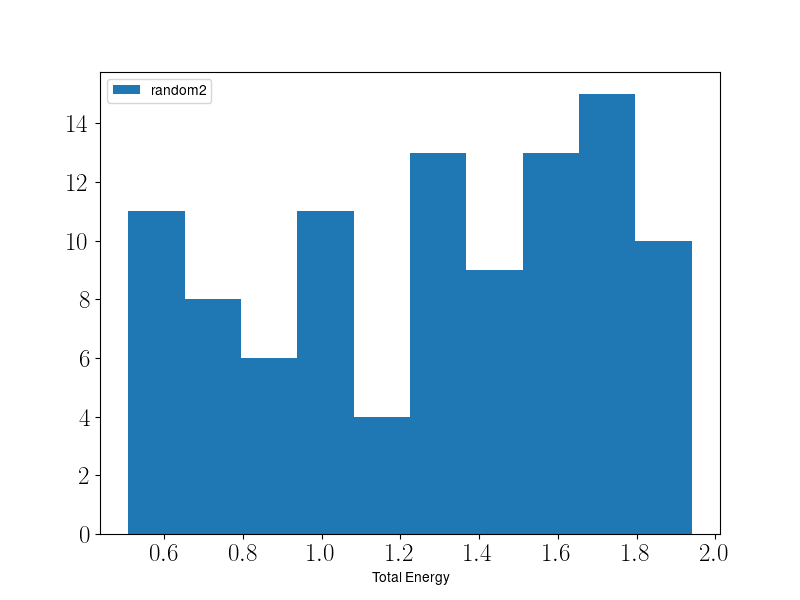
\includegraphics[width=\linewidth]{total}
%        \caption{g = 0}
%		\label{fig:a}
%    \end{subfigure}
%    \caption{Total energy distributions of the generated solution for different %interaction parameter values.}
%\label{fig:energy_dist}
%\end{figure}


\section{Machine Learning}
\subsection{Network architecture}
\noindent Architecture of the network.\\
    A general figure like in the ML\&SE article that describes the work done.\\
    Another figure about internals of the network such as number of layers, how interaction parameter is introduced to the network etc.\\
    Hyperparameters.\\
\subsection{Training}
\noindent    Detailed info about dataset (energy distribution etc).\\
    Indicate that if there is any method to increase the number of examples in low and high energy values.

\subsection{Results}

\section{Inverse Problem}

\clearpage
\section{Conclusion and Discussion}
\subsection{Conclusion}
\subsection{Discussion}
\subsection{Effects of random potential generation method}
\subsection{Are there problems in low and high energies compared to the mean}
\subsection{Inverse problem}


\clearpage

\clearpage
\bibliographystyle{ieeetr}
\bibliography{references}


\appendix
\section{APPENDIX A}
\label{ap:scale}

\textbf{Obtaining harmonic trap potential scaling from Eq.~\eqref{eq:GPE_dimensionless}}

$$V(z) \rightarrow V(\widetilde{z}) \rightarrow \widetilde{V}(\widetilde{z})$$

$$V(z) = \frac{1}{2}m\omega^2 (z-z_0)^2$$

$$V(\widetilde{z}) = \frac{1}{2}m\omega^2 \beta^2 L^2 (\widetilde{z}-\widetilde{z_0})^2$$

$$\widetilde{V}(\widetilde{z}) = \frac{1}{2}(\widetilde{z}-\widetilde{z_0})^2 m\omega^2 \frac{\beta^2 L^2}{\gamma E_0}  $$

The coefficient on the right starts with mass $m$ must be dimensionless. 

$$m\omega^2 \frac{\beta^2 L^2}{\gamma E_0} = 1 $$

$$\beta^2 L^2 = \frac{\gamma E_0}{m\omega^2} $$

In this case, $\alpha$ becomes

$$ \alpha =  \frac{1}{2} \left(\frac{\hbar \omega}{\gamma E_0}\right)^2 $$

Conventionally, $\alpha$ is set to $1/2$, therefore;

$$ \hbar \omega = \gamma E_0 $$

$$ \beta L = \sqrt{\frac{\hbar}{m\omega^2}} $$ 

$ \beta L $ is generally defined as harmonic oscillator length $\ell$

$$ \ell = \sqrt{\frac{\hbar}{m\omega^2}} $$ 

$$ \widetilde{\mu} = \frac{\mu}{\hbar \omega} $$ 

$$ \widetilde{g} = \frac{g}{\hbar \omega \ell} $$

Finally, dimensionless GPE scaled for harmonic trapping potential can be 

$$\widetilde{\mu} \widetilde{\psi} = -\frac{1}{2}\frac{d^2\widetilde{\psi}}{d\widetilde{z}^2} + \frac{1}{2}\widetilde{z}^2\widetilde{\psi} + \widetilde{g}|\widetilde{\psi}|^2 \widetilde{\psi} $$


\end{document}
